\documentclass{article}
\usepackage{color,graphicx,epstopdf}
\usepackage{amsmath,amssymb,amsthm}
\usepackage{xparse}
\usepackage
[
        a4paper,% other options: a3paper, a5paper, etc
        left=4cm,
        right=4cm,
        top=3cm,
        bottom=3cm,
]
{geometry}

% Document Settings
\pagenumbering{arabic}
\title{Linear Statistical Model Assignment 2 -- 2019}
\author{Maleakhi Agung Wijaya, 784091}
\date{Tutor: Qiuyi, Tuesday 3:15 PM}

%%%%%%%%%%%%%%%%%%%%%%%%%%%%%%%%%%%%%%%%%%%%%%%%%%%%%%%%%%%%%%%%%%
% Begin Document
\usepackage{Sweave}
\begin{document}
\maketitle
\Sconcordance{concordance:Assignment2.tex:Assignment2.Rnw:%
1 22 1 1 0 53 1 1 3 2 0 1 1 5 0 1 5 3 0 1 1 14 0 1 2 2 1 1 3 2 0 1 1 9 %
0 1 3 1 0 1 1 1 2 1 1 6 0 1 2 10 1 1 3 12 0 1 2 5 1 1 2 1 0 1 2 7 0 1 2 %
11 1 1 2 1 0 1 3 7 0 1 4 8 0 1 2 5 1 1 2 1 0 2 1 1 3 1 0 3 1 7 0 1 2 23 %
1 1 2 1 0 2 1 4 0 1 2 2 1 1 2 1 0 4 1 4 0 1 2 1 1 1 3 2 0 1 2 21 0 1 2 %
1 3 2 0 1 2 20 0 1 2 1 3 2 0 1 2 19 0 1 2 1 3 2 0 1 2 18 0 1 2 3 1 1 4 %
3 0 1 2 43 0 1 2 4 1 1 3 2 0 1 1 28 0 1 2 1 1 1 3 6 0 1 2 1 1 1 3 6 0 1 %
2 2 1 1 3 6 0 1 2 2 1 1 3 6 0 1 2 20 1 1 2 1 0 4 1 3 0 1 2 1 3 2 0 2 1 %
1 2 1 1 3 0 1 2 1 3 2 0 1 1 9 0 1 2 5 1 1 2 1 0 2 1 1 9 7 0 1 2 4 0 1 2 %
3 1}


% Question One
\section{Question One}
I want to show that the maximum likelihood estimator of the error variance $\sigma^2$ is

\begin{equation*}
    \hat{\sigma} = \frac{SS_{Res}}{n}
\end{equation*}

% Proof
\noindent \textit{Proof:} \\
Assume $\epsilon \sim MVN(0, \sigma^2)$. Then we can calculate the likelihood function by multiplying density of the normal distribution as follows:

% Equation likelihood
\begin{eqnarray*}
    L(\beta, \sigma^2) &=& \prod_{i=1}^n \frac{1}{\sigma\sqrt{2\pi}} e^{-\epsilon_i^2 / 2\sigma^2} \\
    &=& \frac{1}{(2\pi\sigma^2)^{n/2}}e^{-\sum_{i=1}^n\epsilon_i^2/(2\sigma^2)} \\
    &=& \frac{1}{(2\pi\sigma^2)^{n/2}}e^{-(\textbf{y}-X\beta)^T(\textbf{y}-X\beta)/(2\sigma^2)}
\end{eqnarray*}

\noindent We maximise the likelihood by first taking log to create the log-likelihood function and then differentiating it with respect to $\sigma^2$ to find the Maximum Likelihood Estimator for $\sigma^2$:

% Equation log likelihood
\begin{eqnarray*}
    ln L(\beta, \sigma^2) = -\frac{n}{2} ln(2\pi\sigma^2) - \frac{1}{2\sigma^2}(\textbf{y}-X\beta)^T(\textbf{y}-X\beta)
\end{eqnarray*}

% Equation differentiate log likelihood
\begin{eqnarray*}
    \frac{\partial ln L(\beta, \sigma^2)}{\partial \sigma^2} &=& -\frac{n}{2} \frac{1}{2\pi\sigma^2} 4\pi\sigma - \frac{SSRes}{2}\frac{-2}{\sigma^3} \\
    &=& -\frac{n}{\sigma} + \frac{SSRes}{\sigma^3} \\
    &=& 0
\end{eqnarray*}

\noindent Thus, solving the equation above, we have that
\begin{eqnarray*}
    &\rightarrow& \frac{SSRes}{\sigma^3} = \frac{n}{\sigma} \\
    &\therefore& \hat{\sigma^2} = \frac{SSRes}{n}
\end{eqnarray*}

\begin{flushright}
Q.E.D
\end{flushright}

% Question Two
\newpage
\section{Question Two}

\subsection{Part A}
From the question we have that the response variable is \textbf{Cars sold} with the other variables, such as \textbf{Cost}, \textbf{Unemployment rate}, and \textbf{Interest rate} as the predictor variables.

\begin{Schunk}
\begin{Sinput}
> # y
> y <- c(5.5, 5.9, 6.5, 5.9, 8.0, 9.0, 10.0, 10.8)
> print(y)
\end{Sinput}
\begin{Soutput}
[1]  5.5  5.9  6.5  5.9  8.0  9.0 10.0 10.8
\end{Soutput}
\begin{Sinput}
> # X
> X <- cbind(rep(1, length(y)), c(7.2, 10.0, 9.0, 5.5, 9.0, 9.8, 14.5, 8.0), 
+            c(8.7, 9.4, 10, 9, 12, 11, 12, 13.7), 
+            c(5.5, 4.4, 4.0, 7, 5, 6.2, 5.8, 3.9))
> print(X)
\end{Sinput}
\begin{Soutput}
     [,1] [,2] [,3] [,4]
[1,]    1  7.2  8.7  5.5
[2,]    1 10.0  9.4  4.4
[3,]    1  9.0 10.0  4.0
[4,]    1  5.5  9.0  7.0
[5,]    1  9.0 12.0  5.0
[6,]    1  9.8 11.0  6.2
[7,]    1 14.5 12.0  5.8
[8,]    1  8.0 13.7  3.9
\end{Soutput}
\end{Schunk}

\noindent I can calculate the estimate of parameters \textbf{b} by using $\textbf{b} = (X^TX)^{-1}X^T\textbf{y}$. As for variance, it can be computed using $\frac{SSRes}{n-p}.$

\begin{Schunk}
\begin{Sinput}
> # b/ Parameter estimate
> b <- solve(t(X) %*% X, t(X) %*% y)
> print(b)
\end{Sinput}
\begin{Soutput}
           [,1]
[1,] -7.4044796
[2,]  0.1207646
[3,]  1.1174846
[4,]  0.3861206
\end{Soutput}
\begin{Sinput}
> # Variance estimate
> n <- length(y) # number of samples
> p <- dim(X)[2] # number of parameters
> s2 <- sum((y-X%*%b)^2) / (n-p) # SSRes / (n-p)
> print(s2)
\end{Sinput}
\begin{Soutput}
[1] 0.3955368
\end{Soutput}
\end{Schunk}

\noindent $\therefore$ Therefore, we have that \textbf{b} $= \begin{bmatrix}
    -7.4044796\\
    0.1207646\\
    1.1174846\\
    0.3861206
\end{bmatrix}$ and $SSRes = 0.3955368$

\subsection{Part B}
To calculate the covariance of the parameters \textbf{b}, we can inspect the covariance matrix of \textbf{b} which is given by $(X^TX)^{-1}\sigma^2$. However, recall that the question asked about parameters which have the highest covariance in their estimators. This means that we don't need to calculate $\sigma^2$ as it is always greater than 0 by the property of variance (and also since it is the square of $\sigma$). Therefore, we can calculate $(X^TX)^{-1}$ and inspect the off-diagonal column which have the highest magnitude.

\begin{Schunk}
\begin{Sinput}
> # (XTX)-1
> solve(t(X) %*% X)
\end{Sinput}
\begin{Soutput}
            [,1]         [,2]        [,3]         [,4]
[1,] 13.49743324 -0.054817613 -0.69854293 -1.029731987
[2,] -0.05481761  0.024498395 -0.01478859 -0.001937333
[3,] -0.69854293 -0.014788594  0.06226378  0.031714790
[4,] -1.02973199 -0.001937333  0.03171479  0.135362495
\end{Soutput}
\end{Schunk}

\noindent $\therefore$ Therefore, we can see that the entries (1, 4) which correspond to ($\beta_0, \beta_3$) has the highest magnitude of covariance from the matrix given above.

\subsection {Part C}
The 99\% confidence interval can be calculated by using the derived formula $(x^*)^T\textbf{b} \pm t_\frac{\alpha}{2}s\sqrt{(x^*)^T(X^TX)^{-1}(x^*)}$ where $x^*$ is defined as $\begin{bmatrix}1 & 8 & 9 & 5 \end{bmatrix}^T$.

\begin{Schunk}
\begin{Sinput}
> t <- c(1, 8, 9, 5)
> t(t) %*% b + c(-1, 1) * qt(0.995, df=n-p) * sqrt(s2) * 
+   sqrt(t %*% solve(t(X) %*% X) %*% t)
\end{Sinput}
\begin{Soutput}
[1] 3.926075 7.173129
\end{Soutput}
\end{Schunk}

\noindent $\therefore$ Therefore, the confidence interval given by R is $(3.926075, 7.173129)$ or multiplied by thousands, we have the number of cars sold is $(3926.075, 7173.129)$.

\subsection{Part D}
I know from lecture that the prediction interval for the number of cars sold in a year is given by the derived formula of $(x^*)^T\textbf{b} \pm t_\frac{\alpha}{2}s\sqrt{1 + (x^*)^T(X^TX)^{-1}(x^*)}$. Given the interval (4012, 7087), I can calculate the significance level $\alpha$ by rearranging the formula to get $t_\frac{\alpha}{2}$ and later the confidence level used.

\begin{eqnarray*}
  (x^*)^T\textbf{b} + t_\frac{\alpha}{2}s\sqrt{1 + (x^*)^T(X^TX)^{-1}(x^*)} = 7.087 \\
  \rightarrow t_\frac{\alpha}{2} = \frac{7.087 - (x^*)^T\textbf{b}}{s\sqrt{1 + (x^*)^T(X^TX)^{-1}(x^*)}}
\end{eqnarray*}

\noindent Substituting the formula above with our data and calculating with R gives
\begin{Schunk}
\begin{Sinput}
> t.alpha = (7.087 - (t %*% b)) / (sqrt(s2) * sqrt(1 + t %*% solve(t(X) %*% X) %*% t)) 
> # Calculate the confidence level
> pt(t.alpha, n-p)
\end{Sinput}
\begin{Soutput}
          [,1]
[1,] 0.9500215
\end{Soutput}
\begin{Sinput}
> # Thus the confidence level is 90% and we can also check using this
> t(t) %*% b + c(-1, 1) * qt(0.95, df=n-p) * sqrt(s2) * 
+   sqrt(1 + t %*% solve(t(X) %*% X) %*% t)
\end{Sinput}
\begin{Soutput}
[1] 4.012479 7.086724
\end{Soutput}
\end{Schunk}

\noindent $\therefore$ Therefore, we know that the confidence level for the prediction interval is 90\%.

\subsection{Part E}
The model relevance test using a corrected sum of squares uses a hypothesis test in the form of $H_0: \gamma_1 = 0$ with $H_1: \gamma_1 \neq 0$ where $\gamma_1 = \begin{bmatrix} \beta_1 & \beta_2 & \beta_3 \end{bmatrix}^T$ and $\gamma_2 = \beta_0$. The test is given by the test statistics $\frac{R(\gamma_1 | \gamma_2)/(p-1)}{SSRes / (n-p)}$ which follow an F distribution with degree of freedom of $p-1$ and $n-p$. The procedure is given on R below:

\begin{Schunk}
\begin{Sinput}
> H <- X %*% solve(t(X) %*% X) %*% t(X)
> SSReg <- t(y) %*% H %*% y
> SSRes <- sum((y-X%*%b)^2)
> # By theorem, we have that Rg1g2 = SSReg - SSReg(reduced model)
> Rg1g2 <- (SSReg - (sum(y))^2 / n) / (p-1)
> denominator <- SSRes / (n-p)
> Fstats <- Rg1g2 / denominator
> pf(Fstats, p-1, n-p, lower=F) # one tailed test
\end{Sinput}
\begin{Soutput}
            [,1]
[1,] 0.005317255
\end{Soutput}
\end{Schunk}

\noindent $\therefore$ Therefore, the p-value that we have is 0.005317255 and we reject $H_0$ with 5\% significant level.

\section {Question Three}
\textbf{Claim:} $SSRes(Nested Model) \geq SSRes(Full Model)$ \\

\noindent \textit{Proof:} \\
Suppose we have two full rank models in which Model 1 is nested in Model 2. Assume for simplicity without loss of generality that Model 1 has 2 parameters $(\beta_0, \beta_1)$ and Model 2 has 3 parameters $(\beta_0, \beta_1, \beta_2)$. The idea of the proof stay the same for any number of parameters in Model 1 and Model 2 as long as Model 1 is completely nested in Model 2. \\ \\
\textbf{Model 1}: $y_i = b_0 + b_1 x_{i1} + e_i$ \\
\textbf{Model 2}: $y_i = b_0 + b_1 x_{i1} + b_2 x_{i2} + e_i$ \\ \\
Since Model 1 is nested in Model 2, we know that the predictor variables for Model 1 is included in Model 2 along with some other predictor variable not in Model 1 $x_{i2}$. We now define the $SSRes$ as $\sum_{i=1}^n e_i^2 = (y - \widehat{E[y_i]})^2$ where $\widehat{E[y_i]} = b_0 + b_1 x_{i1} + ... +b_n x_{in}$.\\ \\
$\rightarrow SSRes($\textbf{Model 1}): $(y_i - b_0 - b_1 x_{i1})^2 $\\
$\rightarrow SSRes($\textbf{Model 2}): $(y_i - b_0 - b_1 x_{i1} - b_2 x_{i2})^2 $ \\ \\
Estimators for parameters in Model 1 can be obtained using the standard derived formula $(X^TX)^{-1}X^T\textbf{y}$. Now, by choosing the exact same value for $b_0, b_1$ and make $b_2 = 0$, we have obtained that $SSRes(Model1) = SSRes(Model2)$. For other values of $b_2$ (non-zero), it is always possible to optimise and therefore get a lower $SSRes$. This proof holds for general number of predictor variables as long as Model 1 is nested in Model 2.

\begin{flushright}
Q.E.D
\end{flushright}

% Question 4
\section{Question Four}
\subsection{Part A}
I will plot the linear model (without any transformation) with murder rate as response variable and other variables as predictor variables using \lstinline{pairs} command in R that are shown below. The model is given by $Murder = \beta_0 + \beta_1 Population + \beta_2 Income + \beta_3 Illiteracy + \beta_4 Life.Exp + \beta_5 HS.Grad + \beta_6 Frost + \beta_7 Area$.\\

\begin{Schunk}
\begin{Sinput}
> data(state)
> statedata <- data.frame(state.x77, row.names=state.abb, check.names=TRUE)
> pairs(statedata)
\end{Sinput}
\end{Schunk}
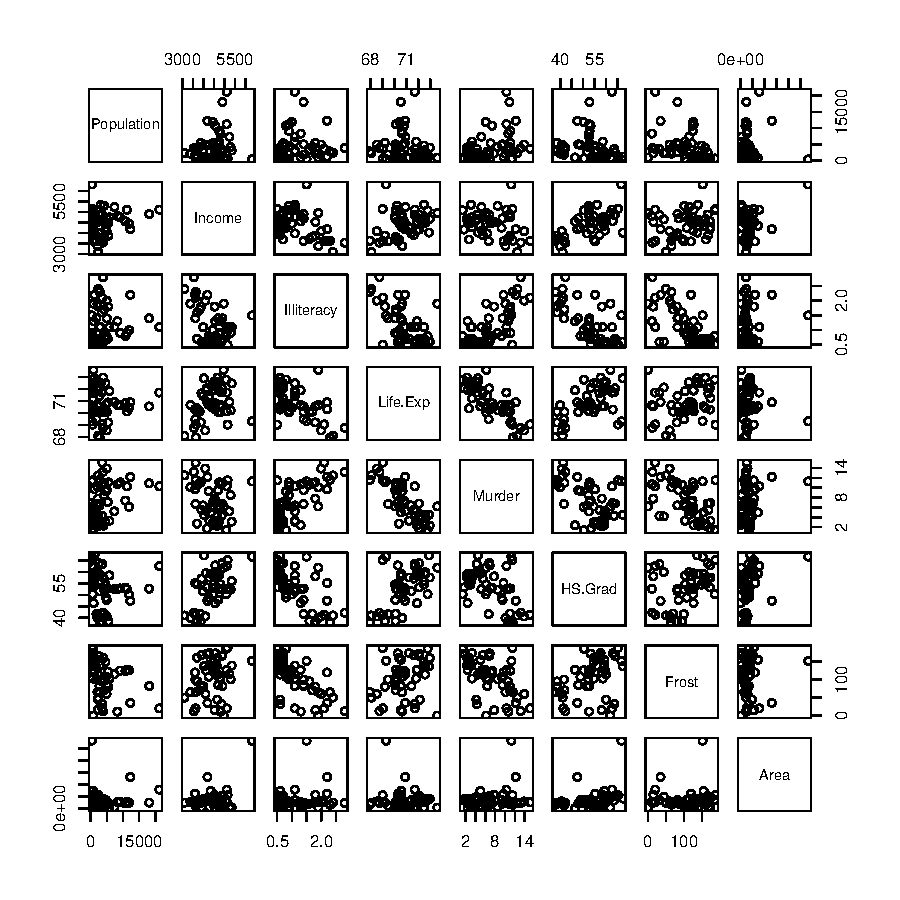
\includegraphics{Assignment2-007}

\noindent If we observe relationship between \lstinline{Murder} and other predictor variables, it can be seen that there are some evidence of heteroskesdasticity in \lstinline{Murder}, especially against \lstinline{population}, \lstinline{income}, \lstinline{HS.Grad}, and \lstinline{Area}. One solution of the problem is to consider taking logs of these variables and check it log transformation improved the fit. Apart from looking at the pairs plot, we can verify it using diagnostic plot 3 to search for signs of heteroskesdasticity which I also found in these variables that are mentioned above. Based on the observation, the new model is given by $Murder = \beta_0 + \beta_1 log(Population) + \beta_2 log(Income) + \beta_3 Illiteracy + \beta_4 Life.Exp + \beta_5 log(HS.Grad) + \beta_6 Frost + \beta_7 log(Area)$. The new pairs plot are shown below using R:

\begin{Schunk}
\begin{Sinput}
> statedata$Population <- log(statedata$Population)
> statedata$Income <- log(statedata$Income)
> statedata$HS.Grad <- log(statedata$HS.Grad)
> statedata$Area <- log(statedata$Area)
> pairs(statedata)
\end{Sinput}
\end{Schunk}
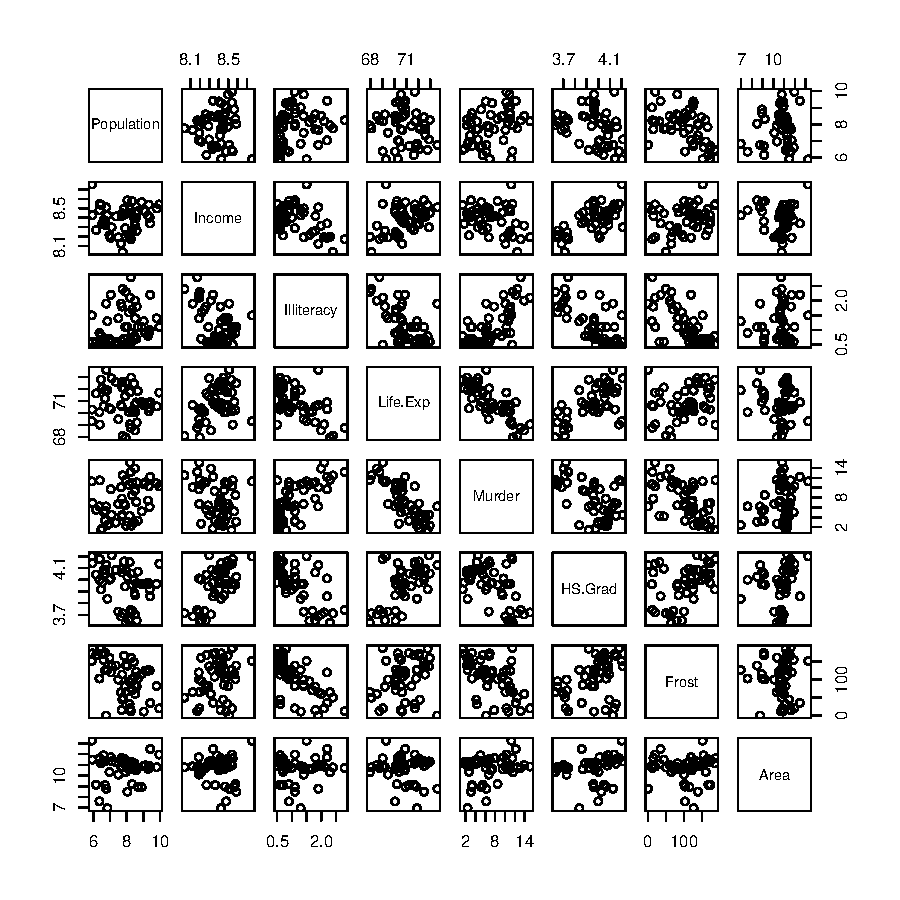
\includegraphics{Assignment2-008}

\subsection{Part B}
\begin{Schunk}
\begin{Sinput}
> # Start with an empty model
> basemodel <- lm(Murder ~ 1, data=statedata)
> add1(basemodel, scope= ~ . + Population + Income + Illiteracy + Life.Exp + HS.Grad + 
+        Frost + Area, test="F")
\end{Sinput}
\begin{Soutput}
Single term additions

Model:
Murder ~ 1
           Df Sum of Sq    RSS     AIC F value    Pr(>F)    
<none>                  667.75 131.594                      
Population  1     86.37 581.37 126.668  7.1313 0.0103090 *  
Income      1     48.01 619.74 129.864  3.7181 0.0597518 .  
Illiteracy  1    329.98 337.76  99.516 46.8943 1.258e-08 ***
Life.Exp    1    407.14 260.61  86.550 74.9887 2.260e-11 ***
HS.Grad     1    175.44 492.31 118.354 17.1052 0.0001414 ***
Frost       1    193.91 473.84 116.442 19.6433 5.405e-05 ***
Area        1     58.63 609.12 128.999  4.6201 0.0366687 *  
---
Signif. codes:  0 '***' 0.001 '**' 0.01 '*' 0.05 '.' 0.1 ' ' 1
\end{Soutput}
\end{Schunk}

\begin{Schunk}
\begin{Sinput}
> # Add Life.Exp as it has the smallest p value
> model2 <- lm(Murder ~ Life.Exp, data=statedata)
> add1(model2, scope= ~ . + Population + Income + Illiteracy + HS.Grad + 
+        Frost + Area, test ="F")
\end{Sinput}
\begin{Soutput}
Single term additions

Model:
Murder ~ Life.Exp
           Df Sum of Sq    RSS    AIC F value    Pr(>F)    
<none>                  260.61 86.550                      
Population  1    50.862 209.75 77.694 11.3972 0.0014838 ** 
Income      1     0.782 259.83 88.399  0.1414 0.7085864    
Illiteracy  1    60.549 200.06 75.329 14.2249 0.0004533 ***
HS.Grad     1     1.864 258.74 88.191  0.3387 0.5633893    
Frost       1    80.104 180.50 70.187 20.8575 3.576e-05 ***
Area        1    30.223 230.38 82.386  6.1656 0.0166517 *  
---
Signif. codes:  0 '***' 0.001 '**' 0.01 '*' 0.05 '.' 0.1 ' ' 1
\end{Soutput}
\end{Schunk}

\begin{Schunk}
\begin{Sinput}
> # Add Frost as it has the smallest p value
> model3 <- lm(Murder ~ Life.Exp + Frost, data=statedata)
> add1(model3, scope= ~ . + Population + Income + Illiteracy + HS.Grad + 
+        Area, test ="F")
\end{Sinput}
\begin{Soutput}
Single term additions

Model:
Murder ~ Life.Exp + Frost
           Df Sum of Sq    RSS    AIC F value   Pr(>F)   
<none>                  180.50 70.187                    
Population  1   12.2130 168.29 68.684  3.3382 0.074179 . 
Income      1    5.1077 175.40 70.751  1.3396 0.253084   
Illiteracy  1    6.0663 174.44 70.477  1.5997 0.212315   
HS.Grad     1    1.5160 178.99 71.765  0.3896 0.535589   
Area        1   30.9733 149.53 62.774  9.5283 0.003422 **
---
Signif. codes:  0 '***' 0.001 '**' 0.01 '*' 0.05 '.' 0.1 ' ' 1
\end{Soutput}
\end{Schunk}

\begin{Schunk}
\begin{Sinput}
> # Add Area as it has the smallest p value
> model4 <- lm(Murder ~ Life.Exp + Frost + Area, data=statedata)
> add1(model4, scope= ~ . + Population + Income + Illiteracy + HS.Grad,
+      test ="F")
\end{Sinput}
\begin{Soutput}
Single term additions

Model:
Murder ~ Life.Exp + Frost + Area
           Df Sum of Sq    RSS    AIC F value  Pr(>F)  
<none>                  149.53 62.774                  
Population  1    9.1315 140.40 61.623  2.9268 0.09401 .
Income      1    4.6252 144.91 63.203  1.4364 0.23700  
Illiteracy  1    8.7371 140.79 61.764  2.7925 0.10165  
HS.Grad     1    0.2798 149.25 64.680  0.0844 0.77280  
---
Signif. codes:  0 '***' 0.001 '**' 0.01 '*' 0.05 '.' 0.1 ' ' 1
\end{Soutput}
\end{Schunk}

\noindent Here we stop since none of the test is significant anymore. Therefore the parsimonious model using Forward Selection includes Life.Exp, Frost, and Area variables (necessary log transformation already applied).

\subsection{Part C}
\begin{Schunk}
\begin{Sinput}
> #Start with a full model
> model <- lm(Murder ~ Population + Income + Illiteracy + Life.Exp + 
+               HS.Grad + Frost + Area, data=statedata)
> step(model, scope= ~ . + Population + Income + Illiteracy + 
+        Life.Exp + HS.Grad + Frost + Area)
\end{Sinput}
\begin{Soutput}
Start:  AIC=59.89
Murder ~ Population + Income + Illiteracy + Life.Exp + HS.Grad + 
    Frost + Area

             Df Sum of Sq    RSS    AIC
- HS.Grad     1     0.324 120.61 58.027
- Income      1     3.555 123.84 59.349
<none>                    120.29 59.893
- Frost       1     5.965 126.25 60.313
- Population  1     8.681 128.97 61.377
- Illiteracy  1    16.334 136.62 64.259
- Area        1    23.023 143.31 66.649
- Life.Exp    1   121.281 241.57 92.756

Step:  AIC=58.03
Murder ~ Population + Income + Illiteracy + Life.Exp + Frost + 
    Area

             Df Sum of Sq    RSS    AIC
<none>                    120.61 58.027
- Frost       1     7.026 127.64 58.858
- Income      1     7.764 128.37 59.146
- Population  1     9.353 129.96 59.761
+ HS.Grad     1     0.324 120.29 59.893
- Illiteracy  1    17.237 137.85 62.706
- Area        1    31.121 151.73 67.504
- Life.Exp    1   135.168 255.78 93.615

Call:
lm(formula = Murder ~ Population + Income + Illiteracy + Life.Exp + 
    Frost + Area, data = statedata)

Coefficients:
(Intercept)   Population       Income   Illiteracy     Life.Exp        Frost  
   80.91395      0.48522      3.33504      1.71612     -1.60172     -0.01123  
       Area  
    0.69099  
\end{Soutput}
\end{Schunk}

\noindent Here we stop since AIC cannot get lower than 58.03. Using stepwise selection with AIC, we have that the final stepwise model only includes Population, Income, Illiteracy, Life.Exp, Frost, and Area as predictor variables.

\subsection{Part D}
The final fitted model is given by $Murder = \beta_0 + \beta_1log(Population) + \beta_2log(Income) + \beta_3Illiteracy + \beta_4Life.Exp + \beta_6Frost + \beta_7log(Area)$. The final model is calculated using stepwise selection with the AIC criterion as it is generally better than forward or backward selection.
\begin{Schunk}
\begin{Sinput}
> final.model <- lm(Murder ~ Population + Income + Illiteracy + Life.Exp + Frost + 
+      Area, data=statedata)
> summary(final.model)
\end{Sinput}
\begin{Soutput}
Call:
lm(formula = Murder ~ Population + Income + Illiteracy + Life.Exp + 
    Frost + Area, data = statedata)

Residuals:
    Min      1Q  Median      3Q     Max 
-2.8885 -1.1825 -0.1014  1.0411  3.3092 

Coefficients:
             Estimate Std. Error t value Pr(>|t|)    
(Intercept) 80.913952  22.973613   3.522  0.00103 ** 
Population   0.485224   0.265725   1.826  0.07479 .  
Income       3.335044   2.004583   1.664  0.10344    
Illiteracy   1.716124   0.692278   2.479  0.01718 *  
Life.Exp    -1.601719   0.230732  -6.942 1.56e-08 ***
Frost       -0.011235   0.007099  -1.583  0.12083    
Area         0.690991   0.207446   3.331  0.00178 ** 
---
Signif. codes:  0 '***' 0.001 '**' 0.01 '*' 0.05 '.' 0.1 ' ' 1

Residual standard error: 1.675 on 43 degrees of freedom
Multiple R-squared:  0.8194,	Adjusted R-squared:  0.7942 
F-statistic: 32.51 on 6 and 43 DF,  p-value: 1.898e-14
\end{Soutput}
\end{Schunk}

\subsection{Part E}
\begin{Schunk}
\begin{Sinput}
> # Plot (which = 1)
> plot(final.model, which=1)
\end{Sinput}
\end{Schunk}
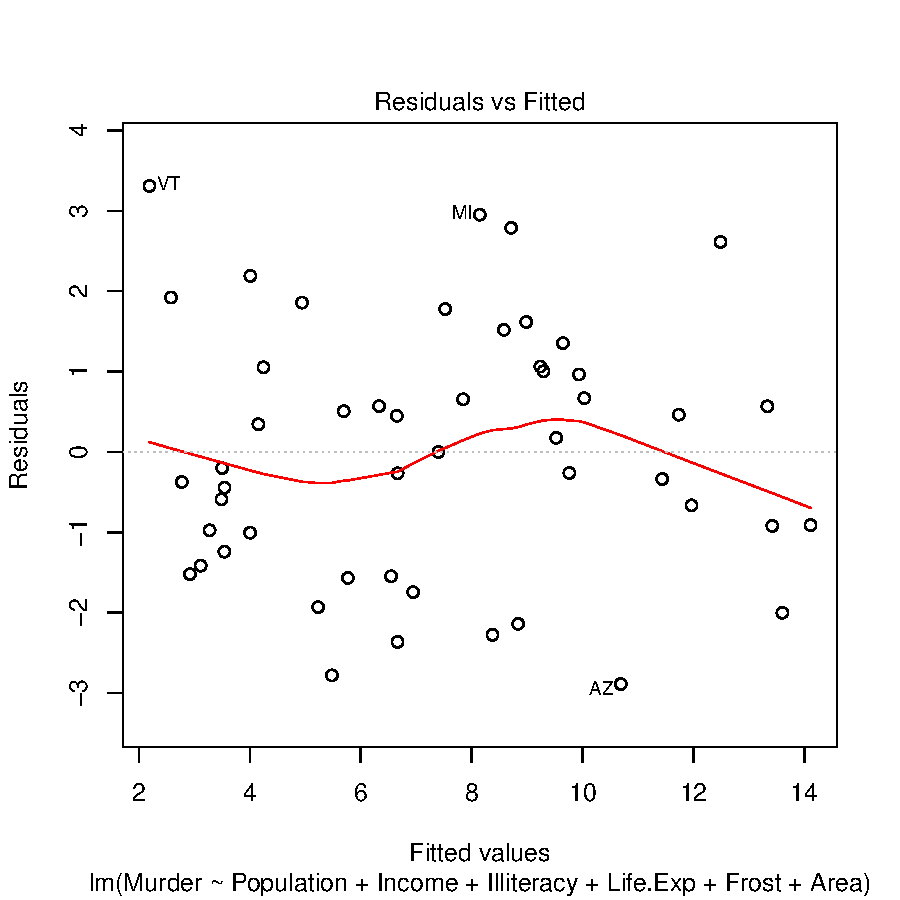
\includegraphics{Assignment2-015}

\noindent The plot here looks good enough since the residual mean is close to 0. Despite that we can see a trend in the plot, it is not enough to be a problem.
\begin{Schunk}
\begin{Sinput}
> # Plot (which = 2)
> plot(final.model, which=2)
\end{Sinput}
\end{Schunk}
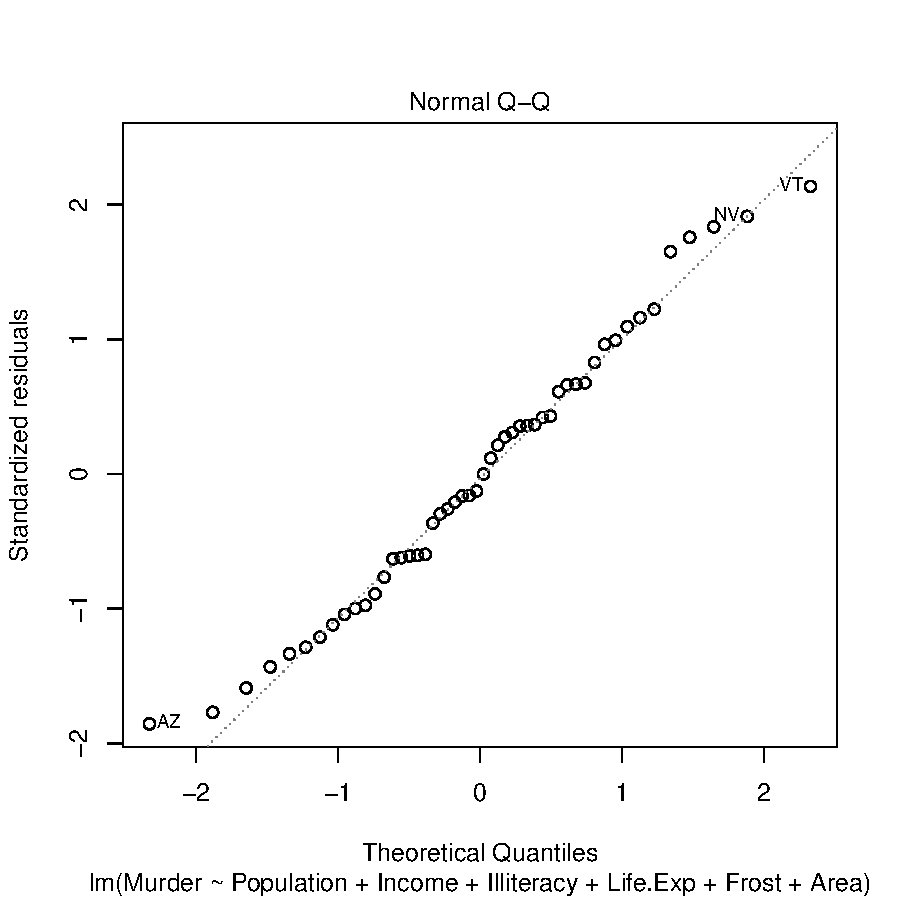
\includegraphics{Assignment2-016}

\noindent The plot looks good as the residual closely follows Normal Distribution.

\begin{Schunk}
\begin{Sinput}
> # Plot (which = 3)
> plot(final.model, which=3)
\end{Sinput}
\end{Schunk}
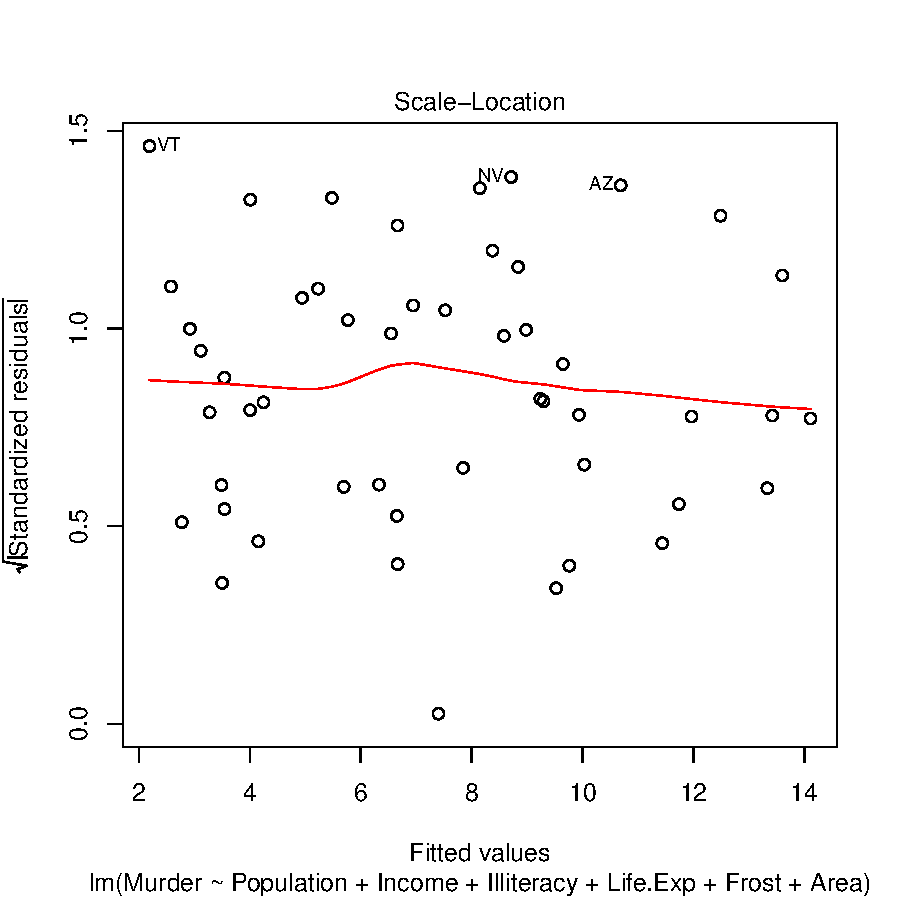
\includegraphics{Assignment2-017}

\noindent The plot also looks good since no sign of heteroskesdasticity and small magnitude of residuals.

\begin{Schunk}
\begin{Sinput}
> # Plot (which = 5)
> plot(final.model, which=5)
\end{Sinput}
\end{Schunk}
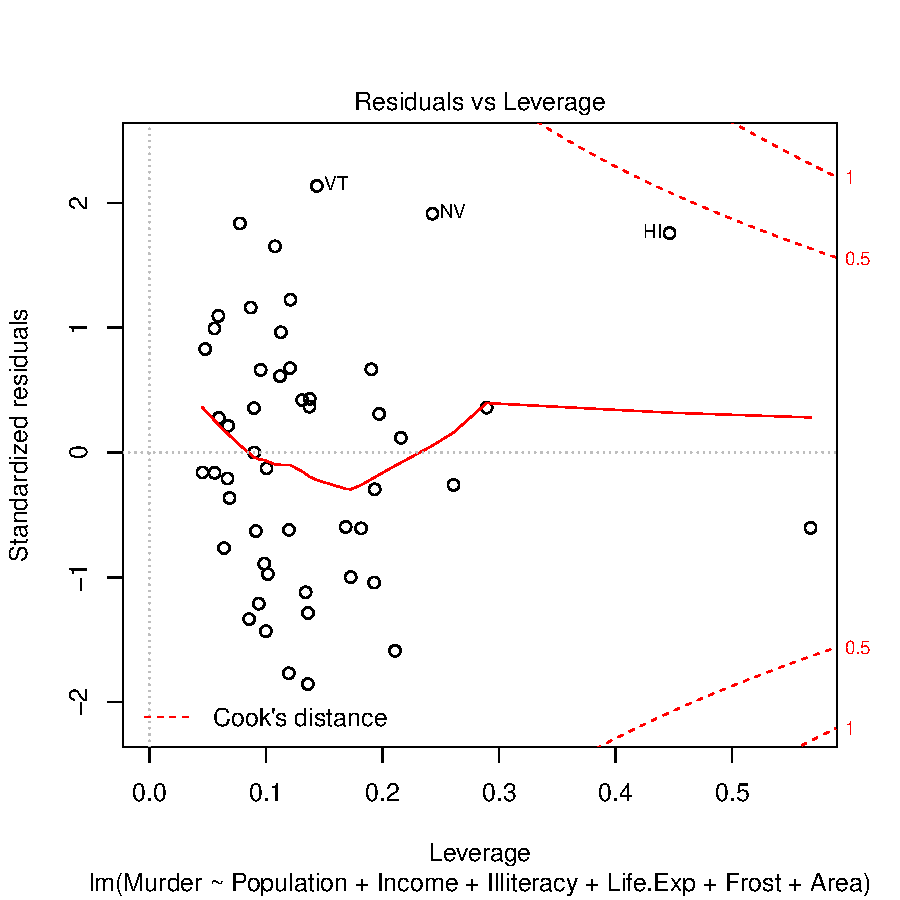
\includegraphics{Assignment2-018}

\noindent The plot looks good as no points with a really high Cook's Distance (< 0.5).

% Question 5
\section{Question Five}
\subsection{Part A}
We know that $\sum_{i=1}^ne_i^2 + \lambda\sum_{j=0}^kb_j^2 = \textbf{e}^T\textbf{e} + \lambda \textbf{b}^T\textbf{b}$. Then we can minimise the function with respect to \textbf{b} by taking partial derivative with respect to \textbf{b}.

\begin{align*}
  \rightarrow \frac{\partial (y-Xb)^T(y-Xb) + \lambda b^Tb}{\partial b} = 0 \\
  \rightarrow \frac{\partial[y^Ty - 2y^TXb + b^TX^TXb + \lambda b^Tb]}{\partial b} = 0 & \text{, since $y^TXb$ is a scalar (okay to transpose)} \\
  \rightarrow -2y^TX + 2X^TXb + 2\lambda b = 0 & \text{, since derivative $y^TAy = Ay + A^Ty$}\\
  \rightarrow (X^TX + \lambda I)b = X^Ty  \\
  \therefore b = (X^TX + \lambda I)^{-1}X^Ty
\end{align*}
\begin{flushright}
Q.E.D
\end{flushright}

\subsection{Part B}
The parameter estimate can be calculated by the formula given on part (a). It is calculated in R as follows:
\begin{Schunk}
\begin{Sinput}
> y <- c(5.5, 5.9, 6.5, 5.9, 8, 9, 10, 10.8)
> cost <- c(7.2, 10, 9, 5.5, 9, 9.8, 14.5, 8)
> unemployment.rate <- c(8.7, 9.4, 10.0, 9.0, 12.0, 11.0, 12.0, 13.7)
> interest.rate <- c(5.5, 4.4, 4, 7, 5, 6.2, 5.8, 3.9)
> lambda <- 0.5
\end{Sinput}
\end{Schunk}

\begin{Schunk}
\begin{Sinput}
> # Scale the response and predictor variables
> cost <- scale(cost, center=TRUE, scale=TRUE)
> unemployment.rate <- scale(unemployment.rate, center=TRUE, scale=TRUE)
> interest.rate <- scale(interest.rate, center=TRUE, scale=TRUE)
> y <- scale(y, center=TRUE, scale=FALSE)
> X <- cbind(cost, unemployment.rate, interest.rate)
\end{Sinput}
\end{Schunk}

\begin{Schunk}
\begin{Sinput}
> # Calculate parameter estimates
> b <- solve(t(X) %*% X + lambda * diag(3)) %*% t(X) %*% y
> print(b)
\end{Sinput}
\begin{Soutput}
          [,1]
[1,] 0.3494789
[2,] 1.7899861
[3,] 0.3432961
\end{Soutput}
\end{Schunk}

\noindent $\therefore$ Therefore, $\textbf{b} = \begin{bmatrix}0.3494789 \\ 1.7899861 \\ 0.3432961\end{bmatrix}$.

\subsection{Part C}
To calculate the optimal value for the penalty parameter $\lambda$, we can minimise the AIC function that is given on the assignment problem. We use R to iteratively find a good solution for $\lambda$ and plot $\lambda$ against AIC.

\begin{Schunk}
\begin{Sinput}
> lambda_S <- c()
> AIC_S <- c()
> n <- 8  # number of data
> for (lambda in seq(0, 1, length=10)) {
+   df <- sum(diag(X %*% solve(t(X) %*% X + lambda * diag(3)) %*% t(X)))
+   b <- solve(t(X) %*% X + lambda * diag(3)) %*% t(X) %*% y
+   SSRes <- sum((y - X %*% b)^2)
+   AIC <- n * log(SSRes/n) + 2 * df
+   lambda_S <- c(lambda_S, lambda) # put new lambda value
+   AIC_S <- c(AIC_S, AIC) # put new AIC value
+ }
> plot(AIC_S, lambda_S, main="Lambda vs AIC")
\end{Sinput}
\end{Schunk}
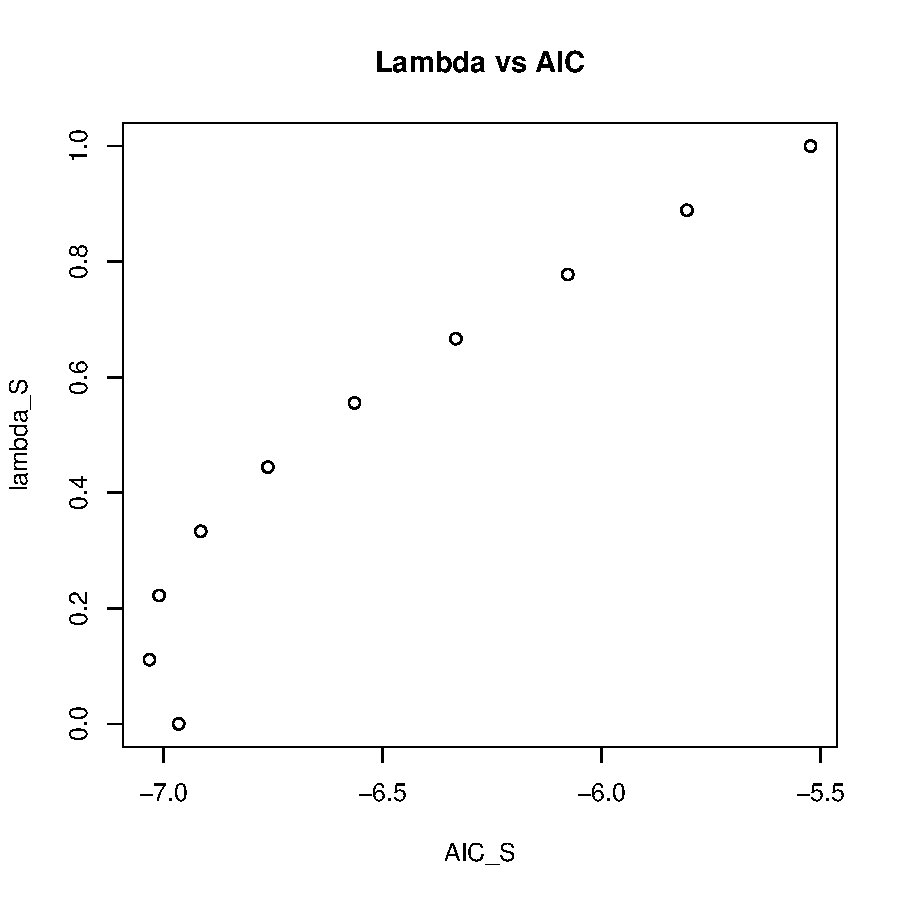
\includegraphics{Assignment2-022}

\noindent $\therefore$ From the plot, we can see that the lowest AIC which indicate the most optimal $\lambda$ is given by a value of $\lambda$ approximately 0.1.

\end{document} 
